\chapter{Calibración R-scan}\label{RscanCalib}

La alta energía de centro de masa alcanzada en el LHC resulta en la producción de partículas con alto momento transverso, dando acceso al estudio experimental de nuevos regímenes cinemáticos. Cuando partículas pesadas como el bosón W, el Z, el Higgs o el quark top decaen hadrónicamente (por ejemplo, $Z\rightarrow q\Bar{q}$, $W\rightarrow q\Bar{q}$, $t\rightarrow W b \rightarrow q\Bar{q} b$, $H\rightarrow q\Bar{q}$), se detectan usando jets. Cuando el $p_t$ de una partícula pesada está cerca o es menor a su masa en reposo, los productos de su decaimiento se encuentran bien separados (geométricamente) y puede establecerse una correspondencia entre un jet y un partón. En ATLAS la elección estándar para reconstruir jets en esta situación es tomar $R=$0.4. Sin embargo, cuando la partícula pesada cumple que $p_t>>m$ (régimen \textit{boosteado}), los productos de su decaimiento se encuentran muy colimados (ver figura \ref{fig:Boost}), y la reconstrucción estándar comienza a fallar. Para este régimen, jets con parámetro $R$ más grande pueden usarse para englobar a las partículas ``hijas'', o bien con $R$ menores al estándar para tratar de resolverlas. 

Un ejemplo de proceso de nueva física que puede producir objetos pesados boosteados significativamente es el decaimiento del $Z'\rightarrow\,t\Bar{t}$, un bosón de gauge de spin 1 propuesto en varias extensiones al SM (por ejemplo en la teoría \textit{topcolor assisted technicolor} \cite{Tecnicolor}). En la figura \ref{fig:fatjets} se puede ver la separación angular entre el quark $b$ y el bosón $W$, productos del decaimiento de un quark top en eventos simulados de $Z'\rightarrow\,t\Bar{t}$ ($m_{Z'}=$1.6TeV). Se observa que para $p_t^{top}<200$GeV el W y el b están bien separados como para ser reconstruidos por el $R$ estándar. Sin embargo, a medida que aumenta el $p_t^{top}$, la separación rápidamente disminuye y para $p_t^{top}\sim$300GeV en adelante la separación $\Delta\,R(W,b)$ cae por debajo de 0.8, lo que implica que los partones individuales no pueden resolverse usando jets con $R=$0.4. \\

\begin{figure}
    \centering
    \begin{subfigure}[b]{0.53\textwidth}
        \centering
        \includegraphics[width=\textwidth]{images/boost}
        \caption{}
        \label{fig:Boost}
    \end{subfigure}
    \hfill
    \begin{subfigure}[b]{0.42\textwidth}
        \centering
        \includegraphics[width=\textwidth]{images/fatjet}
        \caption{}
        \label{fig:fatjets}
    \end{subfigure}
    \caption{(a) Esquema de decaimiento de un quark top con bajo momento transverso (izquierda) y alto momento transverso (derecha). Los productos del decaimiento se encuentran bien separados angularmente en el primer caso, y colimados en el segundo. (b) Separación angular entre el bosón W y el quark b en decaimientos del quark top $t\rightarrow Wb$, en función del momento transverso del top, en eventos simulados de $Z'\rightarrow t\Bar{t}$ ($m_{Z'=}$1.6TeV)\cite{fatjets}.}
    \label{fig:TopTecni}
\end{figure}

Muchos análisis se beneficiarían al tener acceso a jets reconstruidos con diferente parámetro $R$, es decir, a colecciones de jets de distinto radio. Sin embargo, no es factible brindar una calibración completa para cada colección de jets. En particular, no es factible derivar calibraciones \textit{in-situ} para cada radio puesto que éstas son las que llevan más tiempo en derivarse. El esfuerzo de esta tesis se centra en derivar una calibración \textit{in-situ} (es decir, a partir de los datos recolectados y para ser utilizada también en datos), para colecciones de jets de radios $R=$0.2 y $R=$0.6 parcialmente calibradas, usando como objetos de referencia la colección de Jets $R=$0.4 completamente calibrada según lo descripto en la sección \ref{JetCalib}.   


\section{El Método de \textit{Direct-Matching} para calibraciones R-scan}\label{Rscan}


%Since the reference and probe jets differ only in the radii of the clustering algorithm, they should propagate in the same direction within a certain angular distance to each other.



%El objetivo de la calibración \textit{R-scan} es poder derivar una corrección \textit{in-situ} para colecciones de jets reconstruidas con un $R$ diferente al estándar ($R=$0.4), de ahí el nombre de \textit{R-scan}. 
La idea consiste en aprovechar que se tiene una calibración completa para (calo-)jets reconstruidos con el algoritmo anti-$k_t$ con $R=$0.4 a partir de la escala EM \cite{JESpaper} (en adelante referidos como Ref jets), para calibrar jets reconstruidos con tamaño $R$ distinto de 0.4, para los que no se tiene calibraciones de tipo in-situ (en adelante referidos como R-scan jets), usando la topología del evento para comparar el $p_t$ del Ref jet con el del R-scan jet. En esta tesis se derivaron dos calibraciones R-scan, para jets reconstruidos a partir de la escala LCW con el algoritmo anti-$k_t$ de tamaño $R=$0.2 y $R=$0.6. Estos R-scan jets se calibran con un esquema similar al presentado en la figura \ref{fig:JES} en el sentido de que tienen aplicadas las correcciones de pile-up, origen y la MC+JES, pero carecen de las correcciones GSC y las in-situ.\\  

Una técnica utilizada frecuentemente en la derivación de calibraciones in-situ es el método de balance directo, en el que se hace uso del balance de momento transverso entre un objeto de referencia bien medido y el objeto que se quiere calibrar en eventos de topología \textit{back-to-back}. Acá, se explora otro método, que en principio es menos restrictivo ya que no se requiere una topología back-to-back, al que llamaremos \textit{direct-matching}. En este método, evento a evento, se identifica geométricamente (``matching'') el objeto a calibrar, el R-scan Jet, con el objeto de referencia, el Ref Jet, y se calcula el cociente $\mathcal{R}$ (o \textit{response}), entre ellos: 
$$ \mathcal{R}=\frac{p_t^{Rscan}}{p_t^{Ref}} $$ 
\noindent donde $p_t^{Rscan}$ es el momento transverso del jet de tamaño $R$, y $p_t^{Ref}$ es el momento transverso del jet 0.4 con el que se lo identifica angularmente. La respuesta media se define como la media correspondiente a un ajuste Gaussiano realizado sobre el ``core'' de la distribución de $\mathcal{R}$, bineada en $\eta_{det}^{rscan}$ y $p_t^{rscan}$. Este procedimiento se repite en datos y en simulaciones de MC para construir así la respuesta relativa (\textit{relative response}), también como función de $\eta_{det}^{rscan}$ y $p_t^{rscan}$, y el factor de corrección $\mathcal{C}$ finalmente se obtiene de tomar la inversa de este valor.
$$ \mathcal{C}= \frac{<\mathcal{R}>_{MC}}{<\mathcal{R}>_{Datos}}$$\\
\noindent Como resultado, jets de tamaño $R$ calibrados en base a simulaciones de MC se corrigen con este factor $\mathcal{C}$ para dar cuenta de las diferencias entre MC y datos.\\

%En particular, en esta tesis se buscó derivar una calibración R-scan para jets de bajo momento con la idea de complementar otros estudios en curso, 

Una selección de eventos evidente para realizar este estudio es tomar eventos de muchos jets\footnote{Esta selección resulta evidente por la alta sección eficaz de producción de estos eventos en colisiones $pp$, que resulta órdenes de magnitud mayor a la producción de un $Z$, e incluso mayor a la de $Z+jets$.} (también referidos como eventos de dijets). Una calibración Rscan basada en esta selección ya se encuentra en proceso. Sin embargo, debido a la alta sección eficaz de producción de estos eventos muchos de los triggers que disparan con jets de bajo momento en esta topología están muy pre-escaleados y como consecuencia, estos estudios carecen de buena estadística a bajo momento transverso.

En esta tesis se buscó derivar una calibración R-scan, aplicando el método de \textit{direct-matching}, para jets en eventos de $Z(\rightarrow\mu\mu)+jets$, permitiendo obtener una corrección al momento transverso para jets en un régimen de $17GeV\lesssim p_t \lesssim200GeV$. A ``leading order'' los eventos de Z+Jets se producen por los procesos mostrados en la figura \ref{fig:diagramas}. Así, además de explorar un régimen de momento menor, esta selección de eventos también permite obtener una calibración sobre una muestra con una proporción de quarks y gluones diferente en comparación a la derivada en eventos de dijets. En particular, en este trabajo se estudiaron eventos de $Z\rightarrow \mu\mu$ siguiendo las recomendaciones dadas en la referencias \cite{ZmumuTwiki}\cite{Rebecca} para su selección. 

\begin{figure}[h]
    \centering
    \includegraphics[width =0.7\linewidth]{images/diagramas}
    \caption{ Diagramas de Feynman a \textit{leading order} para la producción de eventos de Z+Jets en colisiones $pp$ (la dirección del tiempo es de izquierda a derecha).}
    \label{fig:diagramas}
\end{figure}


%Due to the steeply falling Z-boson p T spectrum, which limits the number of events at large p T , the Z–jet jet analysis covers a limited momentum range 17 GeV ≤ p T < 250 GeV.

\section{Muestras de MC y Datos utilizados}\label{Muestras}

El set de datos utilizado en esta tesis fue recolectado por el detector ATLAS entre los meses de abril y octubre de 2016. Durante este período el LHC operaba a una energía de centro de masa de $\sqrt{s}=$13TeV para las colisiones $pp$, con intervalos de bunch-crossing de 25 ns. Si bien la luminosidad registrada de ATLAS durante este período se corresponde con lo presentado en la figura \ref{fig:Lumi}, luego de exigir algunos requerimientos de calidad la luminosidad que se corresponde con los datos utilizados es menor. Estos requisitos de calidad para los datos producidos en ATLAS tienen en cuenta tanto el estado del haz como posibles inconvenientes con sub-detectores, como por ejemplo, señales de ruido abruptas o momentos en los que la electrónica debe ser reiniciada para algún componente del detector en particular. Estas situaciones pueden presentarse tanto en la operación estándar como en fallas inesperadas. Sin embargo, como no todos los análisis físicos utilizan todas las componentes del detector, y como éstos inconvenientes suelen ser transitorios, resulta conveniente continuar con la adquisición de datos incluso en estos estados degradados \cite{DataQuality}. A partir de esta información se genera una lista de bloques de luminosidad (LB) en las que se considera que el detector estaba operacional, llamada \textit{Good Runs List} o GRL\cite{GRL}. En esta tesis se utilizaron sólo aquellos bloques aprobados por la GRL, determinando una luminosidad integrada total de 32.9 $fb^{-1}$.
Durante este período de adquisición de datos, la máxima luminosidad instantánea registrada fue de 13.8$\times 10^{33}cm^{-2}s^{-1}$. \\

En cuanto a las simulaciones de MC utilizadas, los datasets fueron producidos centralmente por el framework de simulación de ATLAS\cite{AtlasSimulation}, simulando colisiones $pp$ a $\sqrt{s}=$13TeV. Como muestra nominal se utilizaron eventos de Z($\rightarrow\mu\mu$)+jet generados a next-to-leading order (NLO) en QCD con POWHEG-BOX \cite{Powheg} con el set de PDF CT10\cite{CT10}. La lluvia de partones, el evento subyacente y la hadronización se modelan usando Pythia8 \cite{Pythia} con el set de PDFs CTEQ6L1 y parámetros fijados en la \textit{tune}\footnote{Los parámetros utilizados para modelar el evento subyacente y la física no perturbativa en QCD se derivan de comparar con datos, y se los conoce en conjunto como \textit{tune}.} AZNLO \cite{AZNLO}. Efectos de FSR de QED se modelan usando PHOTOS, el cual genera emisiones de fotones a partir de los eventos ya generados (que no contienen radiación QED), modificando la cinemática de los leptones en el estado final.

Para el estudio de la incerteza proveniente del modelado en el MC, se generaron eventos de Z($\rightarrow \mu\mu$)+jets utilizando el generador Sherpa \cite{Sherpa}, el cual genera elementos de matriz ``multi-leg'' ($2\rightarrow N$, con hasta cinco partones en el estado final) con el set de PDF y \textit{tune} NNPDF3.0 NNLO\cite{NNPDF}. De esta manera, además de variar el elemento de matriz generado, se varía la forma en la que se simula la fragmentación, en la muestra nominal se utiliza el modelo de Lund mientras que en la muestra generada en Sherpa se usa el modelo de Clusters.

%Aca se podría discutir tmb. el hecho de que Powheg se genera segun la distribucion de Zpt, mientras que Sherpa se genera en slices???...o no hace falta ???)

%The number of events decreases exponentially with the jet p T . To achieve a high statistic in the tails of the p T distribution, an enormous number of events would have to be simulated. Therefore the MC simulation is divided into different p T samples (J0-J7) as shown in figure 4.1. For each sample the same number of events are generated and afterwards are renormalised

Los efectos del pile-up en ambas muestras se modelan usando eventos de \textit{minimum-bias} simulados con Pythia8 con la \textit{tune} A2 y el set de PDF MSTW2008LO, los cuales se superponen a los eventos de hard-scattering, dando cuenta del in-time pile-up. El out-of-time pile-up se modela de la misma manera, pero incluyendo un offset en el tiempo de la simulación, considerando el ordenamiento de los bunches en el LHC, para dar cuenta del tiempo de adquisición de la señal. El número de estas colisiones se modela teniendo en cuenta el nivel de pile-up en datos. 


Finalmente, los eventos generados se propagan a través de una simulación completa del detector ATLAS basada en el paquete GEANT4 con el fin de simular las interacciones de las partículas a medida que avanzan sobre el material del detector. El siguiente paso es la conversión de depósitos de energía y $hits$ en el detector en voltajes y corrientes, y la posterior reconstrucción de objetos (usando los mismos algoritmos) tal y como ocurriría en el detector real. 

Para comparar la simulación con los datos experimentales, se calcula un factor de normalización que tiene en cuenta la sección eficaz con la que se generó la muestra, la eficiencia del generador, y la luminosidad en los datos. Aún luego de aplicado este factor, se observó un desacuerdo en la escala de los datos y la muestra de MC. Sin embargo, en este trabajo se requiere conocer la forma de las distribuciones considerando que en el método de estudio las distribuciones para $\mathcal{R}$ se arman de manera independiente para datos y MC, y de ellas se toma la media para obtener el factor de calibración final. En este contexto, se asume que este desacuerdo en la escala entre datos y MC no altera la forma de las distribuciones, y por lo tanto no altera los valores medios a utilizar. Se decidió entonces calcular un factor de escala (x0.8) a aplicar en la muestra (nominal) de MC a partir de la distribución de $<\mu>$ en datos y MC, la cual se estudia luego de considerar selecciones de calidad, y antes de realizar cualquier corte de tipo cinemático. 

\section{Derivando las calibraciones...}\label{Derivandow}

Antes de comenzar con el análisis, se realiza una serie de selecciones iniciales, evento a evento, con el fin de garantizar que los eventos sobre los que se trabaje cumplan algunos requerimientos de calidad, y reducir la cantidad de eventos teniendo en cuenta la física buscada. En la tabla \ref{tab:cut} se muestra un resumen de todos los cortes realizados y su impacto en la cantidad de eventos. Esta selección inicial y la reconstrucción de los objetos y sus calibraciones se realizan en la GRID\footnote{La \textit{Worldwide LHC Computing Grid} (WLCG) es un sistema de almacenamiento y procesado de datos formado por una infraestructura de ordenadores distribuidos globalmente, dando acceso a todos los colaboradores sin importar su ubicación física. La WLCG recibe el apoyo de varias \textit{grids} asociadas a lo largo del mundo, y es coordinada por CERN.}. Luego, a nivel local, se realiza una selección de eventos más específica a la búsqueda de un $Z$, y al método de \textit{direct-matching}. 

Si bien en las simulaciones de MC se trata de reproducir las condiciones de pile-up observadas en datos reales, se asignan pesos adicionales a los eventos en las simulaciones de MC de manera de corregir posibles diferencias residuales en la distribución del número medio de interacciones por bunch-crossing $<\mu>$ en datos reales y en simulaciones \cite{PRW}. En la figura \ref{fig:avgmu} se muestra la distribución para $\mu$ en datos y en la muestra nominal de MC. Esta última además se muestra antes y después de incluir esta corrección por pile-up, observándose un buen acuerdo en la forma de las distribuciones en datos y MC, y un valor para $<\mu>$ centrado aproximadamente en 21 interacciones.

\begin{figure}[ht]
    \centering
    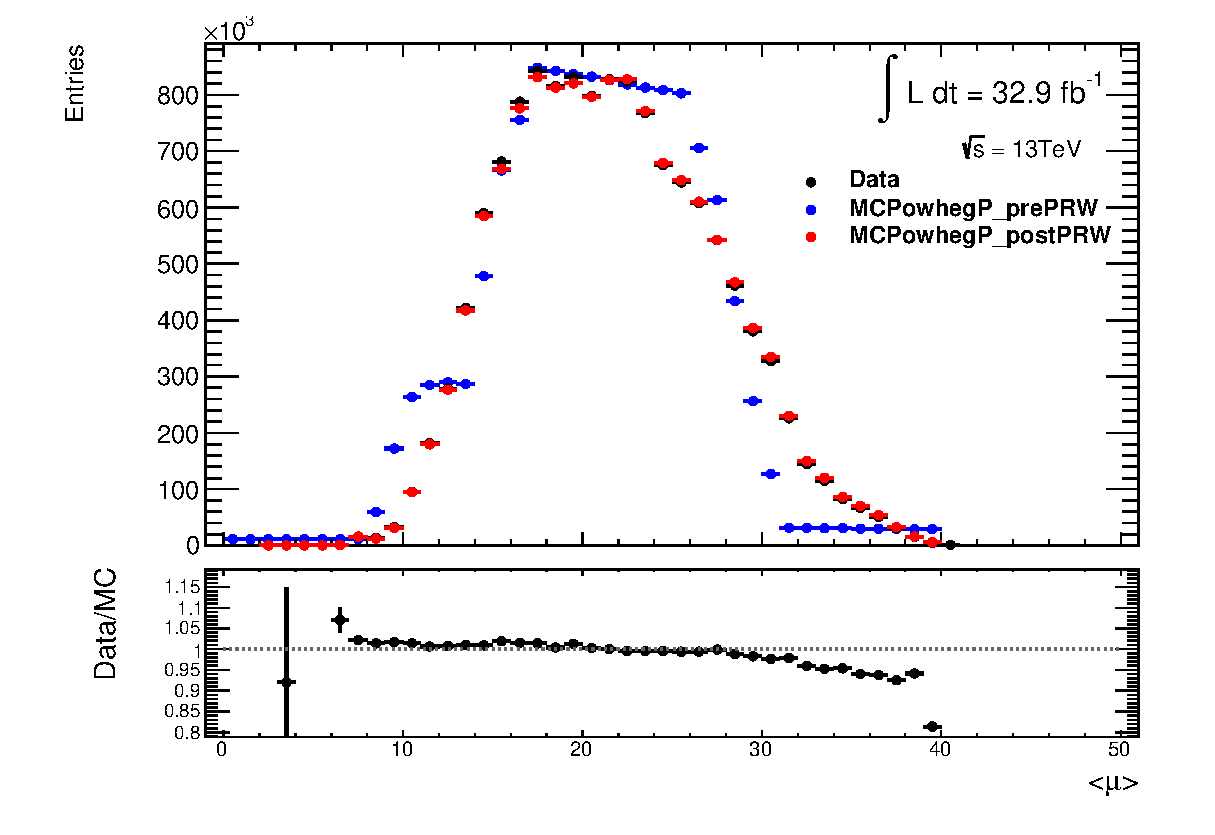
\includegraphics[width =0.9\linewidth]{images/Final_AvgMu}
    \caption{Distribución del número medio de interacciones por bunch crossing (luego de la selección de calidad de datos según la sección \ref{DataQu}) para colisiones $pp$ a $\sqrt{s}=$13TeV para datos recolectados en ATLAS durante 2016 a una luminosidad integrada de 32.9 $fb^{-1}$ (en negro), para la simulación nominal (Powheg $+$ Pythia) antes de la corrección de pile-up (en azul: ``MCPowhegP$\_$prePRW'') y para la simulación nominal luego de la correción de pile-up (en rojo:``MCPowhegP$\_$postPRW''). Algunos puntos negros quedan ocultos bajo puntos rojos. La distribución para los datos tiene una media $\overline{<\mu>}=$21.602$\pm$0.002 con una desviación estándar $\sigma=$5.673$\pm$0.001; y para la muestra simulada nominal luego de la corrección $\overline{<\mu>}=$21.672$\pm$0.001 y $\sigma=$5.709$\pm$0.001. En el panel inferior se puede ver el cociente de ambas distribuciones.}
    \label{fig:avgmu}
\end{figure}

\subsection{Calidad de Datos} \label{DataQu}

El primer paso en esta serie de selecciones tiene que ver con criterios de calidad que se aplican en datos (y cuando se indique también en MC) previo a cualquier recorte de índole cinemático. Estas recomendaciones se usan de base, con algunas excepciones, en todos los análisis de ATLAS y tienen que ver, principalmente, con el estado del detector. 

El primero de estos requerimientos de calidad es que el evento pertenezca a un LB que aparezca en la GRL\footnote{La GRL utilizada: data16$\_$13TeV.periodAllYear$\_$DetStatus-v88-pro20-21$\_$DQDefects-00-02-04$\_$PHYS$\_$StandardGRL$\_$All$\_$Good$\_$25ns.xml}.
Los LB son períodos de adquisición de datos de alrededor de uno o dos minutos, y varios cientos de LB se agrupan en $runs$.
Como ya se mencionó, un grupo encargado de estudiar la calidad de los datos adquiridos por el detector ATLAS produce una lista de aquellos LB registrados que son aptos para su uso en análisis físicos. Partiendo exclusivamente de aquellas runs\footnote{En esta tesis no se utiliza el dataset completo, es decir todas las runs registradas durante el año 2016, puesto que algunas runs serían enteramente descartadas por la GRL. Así, se decidió utilizar como dataset sólo aquellas runs que contengan algunos LB en la GRL.} con algún LB que figuren en la GRL, se tiene que la fracción de eventos considerados como ``buenos'' representa un $\sim 97\%$ de los eventos totales considerados.

El siguiente de los requerimientos tiene que ver con la reconstrucción de los vértices: se pide que en el evento haya al menos un vértice primario. Este criterio se aplica tanto en datos como en MC.

A continuación, en datos, evento a evento se buscan distintas \textit{flags} que alertan acerca del mal funcionamiento de algún sub-detector durante algún período de tiempo. En particular, se buscan flags en los calorímetros LAr, y los de tejas. Distintas señales abruptas y globales de ruido pueden aparecer en estos calorímetros en escalas temporales menores a las de un LB, con lo cual estos eventos no pueden ser excluidos por la GRL. Estos eventos son vetados en este paso.

%PODRIA PONER UN CUTFLOW DE ESTE CLEANING NOMAS..
%PORQUE SI PONGO CON TRIGGER TMB..->el trigger está preescaleado.


\subsection{Trigger}

Con la idea de seleccionar aquellos eventos de $Z\rightarrow \mu\mu$ se pide que los eventos pasen un $OR$ de dos triggers (a nivel HLT) que disparan ante muones, ambos alimentados por un trigger a nivel 1 (L1) del sistema de trigger de muones con umbral de 20GeV. El primero de ellos pide que haya al menos un muón en el evento, de calidad y aislación media con momento transverso por arriba de 26GeV. El segundo trigger considerado requiere que haya al menos un muón en el evento con $p_t>$50GeV.  
En la figura \ref{fig:trigEff} se muestra la eficiencia absoluta y relativa (al trigger L1 mencionado) del $OR$ de los triggers. 

\begin{figure}[ht]
    \centering
    \includegraphics[width =0.7\linewidth]{images/TriggEff1}
    \caption{Eficiencia del trigger de muones en función del $p_t$ del muón (reconstruido a nivel \textit{offline} usando software estándar de ATLAS) en la región del barril del detector. La eficiencia se determina en relación a muones aislados que pasan el criterio de calidad ``Media''. En negro se muestra la eficiencia absoluta del trigger a nivel 1 (L1) con umbral en 20GeV. En azul se muestra la eficiencia absoluta de un $OR$ de triggers que requieren al menos un muón de más de 26Gev y aislación media (determinada usando las trazas en el ID reconstruidas a nivel \textit{online} en el HLT) ó de más de 50GeV. En rojo se muestra la eficiencia de este trigger relativa a la curva negra. Esta eficiencia fue determinada usando el método de \textit{tag-and-probe} en candidatos a eventos de $Z\rightarrow \mu\mu$ (sin substracción de eventos de \textit{background}), en el que uno de los muones se utiliza para disparar el trigger y el otro para medir su eficiencia, en datos recolectados en 2016 a 13TeV. Sólo se muestran las incertezas estadísticas\cite{TrigEff} 
    }
    \label{fig:trigEff}
\end{figure}


Puede observarse que la combinación de triggers alcanza una eficiencia (relativa) cercana a 1 para muones con momento transverso superior a 26GeV.

A su vez, como en las simulaciones de MC resulta imposible tener en cuenta cada detalle del experimento real, cuestión que en última instancia también tiene efecto en la eficiencia del trigger en la simulación, el grupo de ``Muon Combined Performance'' (CP) dentro de ATLAS provee de un factor de corrección a la eficiencia del trigger simulado comparándola con la eficiencia del trigger que se tiene en los datos experimentales\cite{MCPGuidelines}. 

\subsection{Reconstrucción y selección de eventos}

El siguiente paso es la reconstrucción de los muones y los jets. Como ya se mencionó en la sección \ref{Muones}, los muones deben pasar ciertos criterios de calidad. Se seleccionan los eventos que tengan exactamente dos muones (\textit{combined}) de calidad \textit{Medium}\cite{SelTool}, aislados\cite{IsoTool} y con carga opuesta, ambos en el rango $|\eta|<$2.4 y $p_t>$25GeV. De la misma manera que con los triggers, el grupo CP provee de un factor de corrección \cite{MCPGuidelines} a aplicar en simulaciones de MC para dar cuenta de la diferencia entre la 
eficiencia de reconstrucción de los muones en datos experimentales y en las simulaciones. La forma en la que se determina la eficiencia de reconstrucción de los muones se explica en la referencia \cite{MuonReco}. 
\\

Los jets se reconstruyen utilizando el algoritmo anti-$k_t$ a partir de la escala EM para los Ref Jets, y a partir de la escala LCW para los R-scan Jets. Esto quiere decir que en un mismo evento los jets se reconstruyen de tres maneras diferentes ($R=$0.4, 0.2 y 0.6 respectivamente). Las colecciones de jets se calibran evento a evento como ya fue explicado en \ref{Rscan}. En una primera instancia, se rechazan todos los jets con $|y|>$4.4 y los que se encuentren a una distancia angular $\Delta R<$0.35 de cualquiera de los dos muones. 

Además, los eventos también se evalúan considerando la \textit{calidad} de los jets, criterio que se aplica tanto en datos como en MC. Cuando se reconstruyen los eventos, es posible que jets formados con información de los calorímetros sean generados por fuentes \footnote{Por ejemplo, ruido abrupto en el calorímetro, rayos cósmicos u otros backgrounds que no provienen de la colisión.} que nada tienen que ver con el flujo de energía desde el hard scatter. Entonces, la referencia \cite{JetCleaning} propone dos selecciones para identificar estos jets falsos: ``BadLoose'' y ``BadTight'', que tienen en cuenta distintos cocientes de energía (por ejemplo, los cocientes entre la energía depositada en el calorímetro EM o hadrónico y la energía total del jet) y variables que consideran las trazas que dan origen a ese jet (por ejemplo, el cociente entre la suma escalar del $p_t$ de las trazas con origen en el vértice primario y el momento del jet). La primera es la que se usa en este trabajo y  está diseñada para mantener alta la eficiencia de jets ``buenos'' manteniendo la eficiencia de rechazo a los jets falsos lo más alta posible. La estrategia de selección de eventos debido a estos criterios de calidad sobre los jets se aplica solamente a los Ref Jets según las recomendaciones en \cite{JetCleaningTool}, en las que se busca descartar aquellos eventos que tengan algún Ref Jet de tipo ``LooseBad'' pero que no hayan sido etiquetados como pile-up jets. Una cantidad que se utiliza para discriminar jets provenientes del hard scatter de pile-up jets es el coeficiente de \textit{Jet Vertex Tagger} o JVT, el cual pide a los jets con $p_t<$50GeV y $|\eta|<$2.4 que estén asociados con un vértice primario (al \textit{working point} medio de JVT \cite{JVTtool}), identificando el 92$\%$ de hard-scatter jets y el $98\%$ de pile-up jets. La selección de eventos debido a la calidad de los jets entonces descarta aquellos eventos con ``LooseBad'' jets que estén fuera del rango de aplicación del criterio de JVT, y aquellos con ``LooseBad'' jets que JVT identifique como provenientes del hard-scatter. \\ 


\begin{figure}[ht]
    \centering
    \begin{subfigure}[b]{0.495\textwidth}
        \centering
        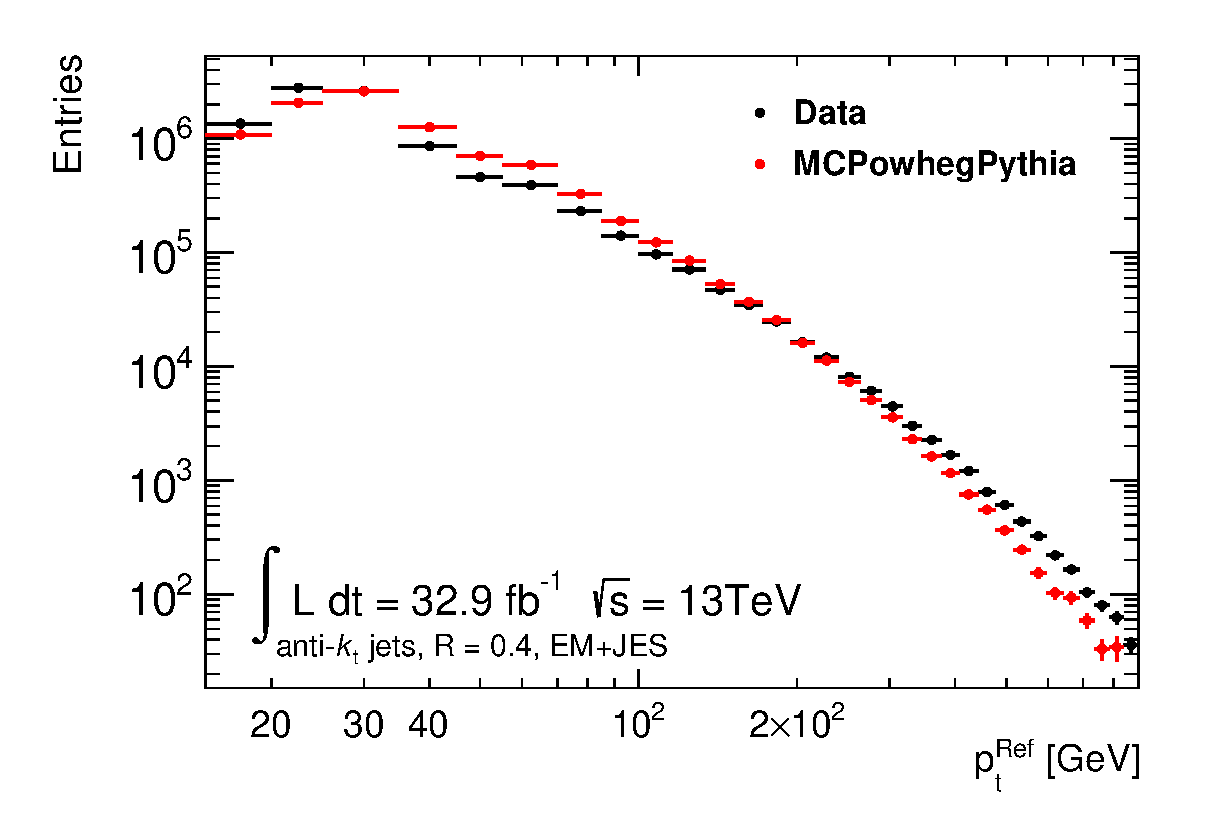
\includegraphics[width=\textwidth]{images/Final_LeadRefPt}
        \caption{ }
        \label{fig:JetptDist}
    \end{subfigure}
    \hfill
    \begin{subfigure}[b]{0.495\textwidth}
        \centering
        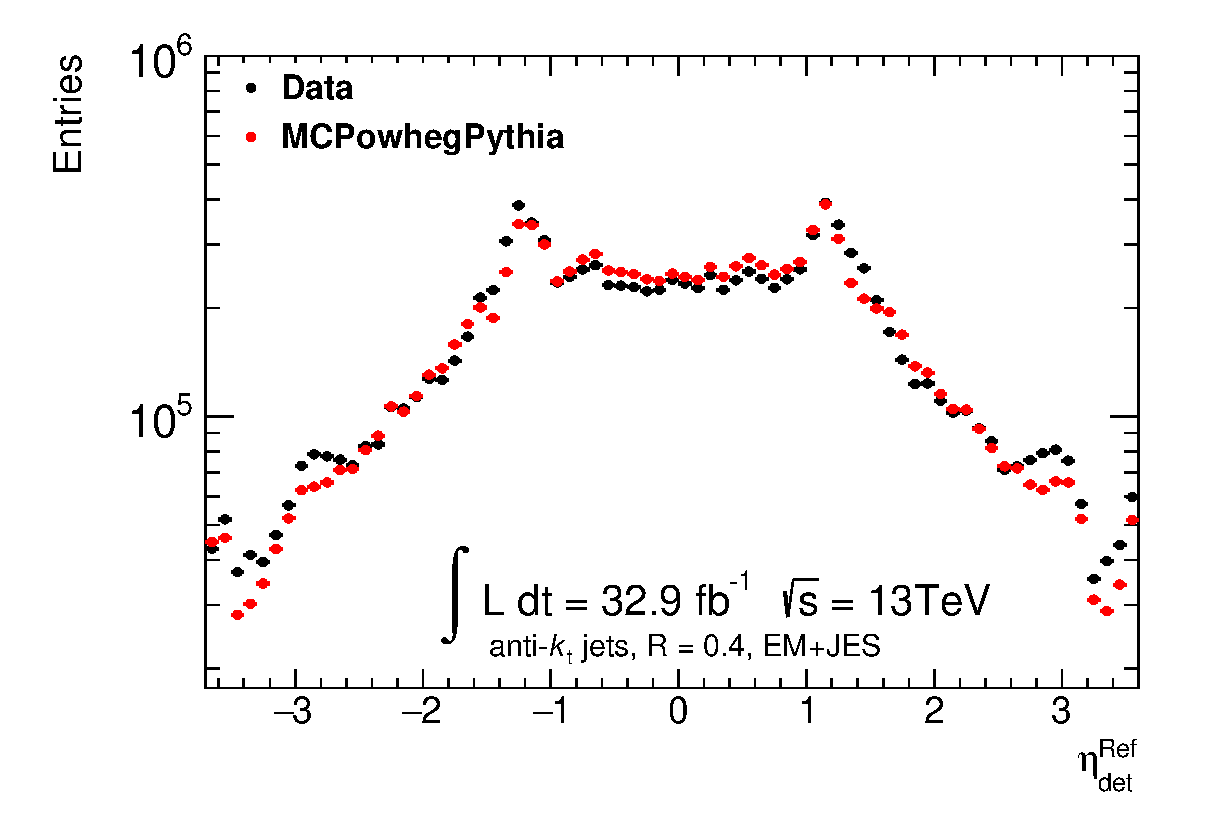
\includegraphics[width=\textwidth]{images/Final_RefLeadEta}
        \caption{}
        \label{fig:JetEtaDist}
    \end{subfigure}
    \caption{ Distribución de (a) $p_t^{Ref}$ y (b) $\eta_{det}^{Ref}$ para datos recolectados en ATLAS en 2016 (en negro) y para la muestra nominal de MC (en rojo), luego de la selección inicial de eventos.}
    \label{fig:JetDistro}
\end{figure}

En la figura \ref{fig:JetDistro} se muestra la distribución del momento transverso del Ref Jet con mayor momento, o \textit{leading} jet, y la distribución de pseudo-rapidez. En ambos casos se muestran las distribuciones tanto en datos como en la muestra nominal de MC.\\ 

El siguiente paso de la selección tiene que ver con seleccionar los eventos que contengan un candidato a $Z$. Para ello se calcula la masa invariante de los dos muones y se seleccionan aquellos eventos tal que la misma sea consistente con la masa de un $Z$: 80GeV$<m_{\mu \mu}<$116GeV. En la figura \ref{fig:Zmass} puede verse la distribución de la masa invariante de los dos muones tanto en datos como en MC. Se observa que la simulación reproduce la forma de la distribución en datos, mostrando una resonancia acorde con un $Z$; y en la figura \ref{fig:Zpt} puede verse la distribución de $p_t$ del $Z$ reconstruido para los eventos seleccionados. 

\begin{figure}[ht]
    \centering
    \begin{subfigure}[b]{0.495\textwidth}
        \centering
        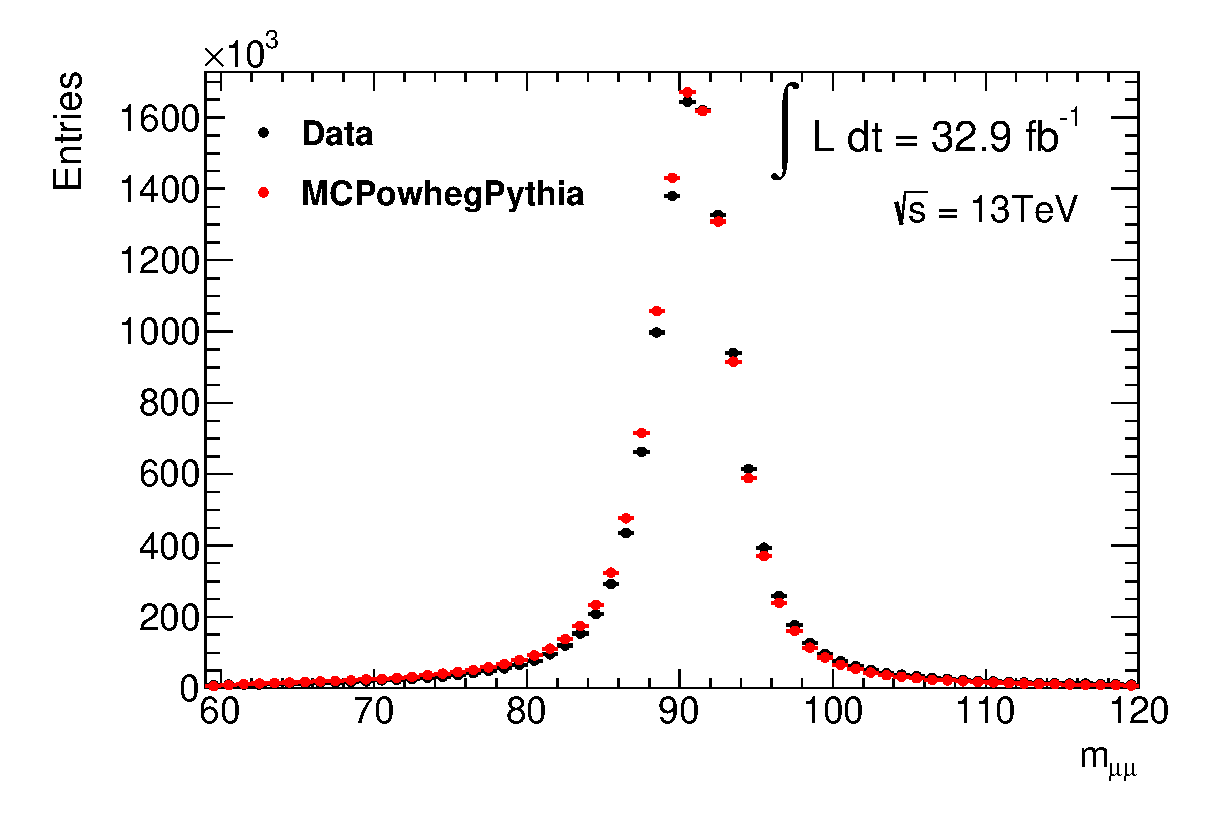
\includegraphics[width=\textwidth]{images/Final_Zmass}
        \caption{}
        \label{fig:Zmass}
    \end{subfigure}
    \hfill
    \begin{subfigure}[b]{0.495\textwidth}
        \centering
        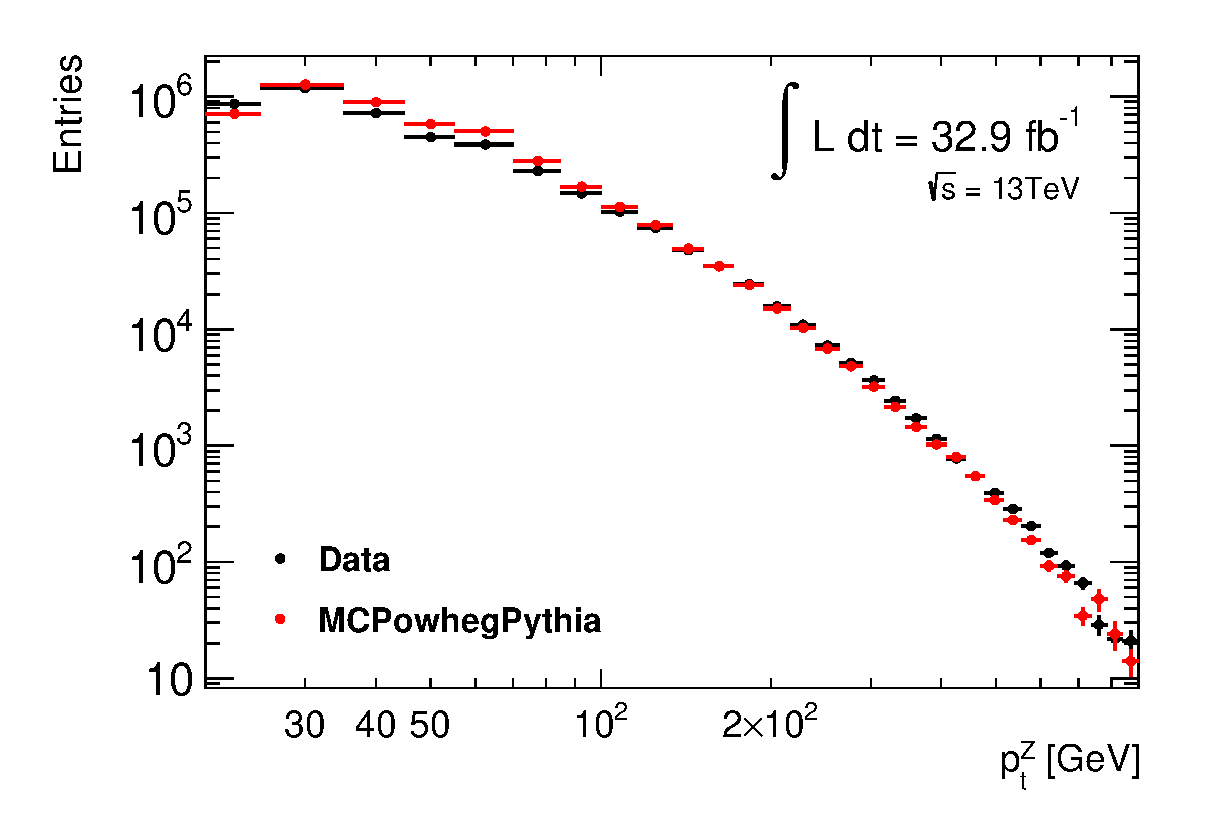
\includegraphics[width=\textwidth]{images/Final_Zpt}
        \caption{}
        \label{fig:Zpt}
    \end{subfigure}
    \caption{ En negro se muestra la distribución correspondiente a los datos recolectados en ATLAS en 2016, aprobados por la GRL, y en rojo se muestra la distribución correspondiente a la muestra de MC nominal (Powheg + Pythia) para (a) la masa invariante del par de muones para los eventos seleccionados, y (b) el $p_t^Z$ resultante luego de la selección de eventos con masa invariante del par de muones consistente con la masa del Z.} 
    \label{fig:Z}
\end{figure}

Finalmente, se descartan aquellos eventos que luego de estos recortes no contengan al menos un R-scan Jet y al menos un Ref Jet.

\subsection{Selección de Jets}

El primer paso para derivar la calibración R-scan es calcular el cociente $\mathcal{R}$. El estudio se realiza primero para la colección de R-scan Jets con un $R$ y luego se repite el procedimiento para el otro. Para poder calcular este cociente primero se requiere de una selección de los jets a utilizar. En la tabla \ref{tab:sel} se resumen los distintos cortes aplicados a las colecciones de jets, indicando su valor nominal, y su variación sistemática cuando corresponda (ver sección \ref{Syst}).

\begin{table}[ht]
    \centering
    \begin{tabular}{|l|l|l|} 
        \hline
        %\multicolumn{2}{|c|}{input} & \multicolumn{2}{c|}{output} & \\
        Selección & Valor Nominal & Variación Sistemática\\ \hline\hline
        Ref Jet $p_t$  & $>15$GeV &\\ \hline
        Ref Jet $\eta$ & $|\eta|<$3 & \\ \hline
        Rscan Jet $p_t$ & $>10$GeV &  \\ \hline
        Rscan Jet $\eta$ & $|\eta|<$3 & \\ \hline
        $\Delta \varphi (Z,jet^{Ref})$ & $|\Delta\varphi|>$1.57 &\\ \hline
        Aislación $\Delta R> f*R$ & $f=2$ & 1.5 ($\downarrow$) 2.5 ($\uparrow$) \\ \hline
        $p_{t,\%}$ & 10 $\%$ & 5$\%$ ($\downarrow$) $20\%$($\uparrow$)  \\ \hline
        JVT & 0.59 & 0.11 ($\downarrow$) 0.91 ($\uparrow$) \\ \hline
        Matching $\Delta R(jet^{Rscan},jet^{Ref})<dR$ & 0.2 & 0.1 ($\downarrow$) 0.3 ($\uparrow$)\\ \hline
    \end{tabular}
    \caption{Resumen de cortes aplicados a los jets durante el proceso de selección en el método de direct-matching para eventos de $Z+jets$.}
    \label{tab:sel}
\end{table}


Como primera medida, se seleccionan los Ref Jets con $p_t>$15GeV, ya que para valores inferiores la JES no está bien definida y, por lo tanto, no se puede decir que el Ref Jet esté bien calibrado como para servir de objeto de referencia para calibrar los R-scan Jets; y que se encuentren en el hemisferio opuesto al Z pidiendo $|\Delta \varphi|>$1.57; y los R-scan con $p_t>$10GeV. Además, se pide que ambos tipos de jets estén en la región $|\eta^{det}|<$3 con la intención de evitar posibles sesgos provenientes del hecho de que el trigger de muones está limitado a $|\eta|<$2.4.\\

%y Ref Jets con eta menor a 3.0 por fisica: para no introducir un bias con Z forward-> mi trigger de muones solo anda en eta central y porque no se necesita estudiar el caso forward

\noindent \textbf{Aislación}:

\indent La calibración dada por este método tiene sentido cuando se trata de jets aislados, de otra forma no se podría hallar una correspondencia entre el R-scan Jet que se identifica angularmente con un Ref Jet. Por ejemplo, podría tenerse el caso en que un R-scan Jet de $R=$0.6 englobe parte de dos Ref Jets. En estos casos, resultaría incorrecto asumir que el $p_t$ de uno de los Ref Jets sirve como referencia para calibrar el momento del R-scan Jet. El criterio de aislación aplicado utiliza distinto umbral cuando se trata de pedir aislación para RefJet-RefJet y RscanJet-RscanJet, ya que tiene en cuenta que justamente los jets tienen distinto tamaño. Entonces, se guardan aquellos jets que verifican $\Delta R >f*R$, donde $\Delta R$ se calcula entre jets de la misma colección, $R$ es el radio de la colección, y $f$ un factor, que en el caso nominal vale 2, que determina qué tan separados deben estar los centros de los jets en  unidades de $R$. Como el discriminante se calcula de a pares de jets, no se descartan automáticamente ambos jets si resultara que no están aislados, sino que se tiene en cuenta la relación entre los momentos de ambos jets. Es decir, se descarta el de menor momento ($p_{t,1}$), y para decidir sobre el de mayor momento($p_{t,2}$) se tiene en cuenta qué porcentaje, ($p_{t_{\%}}$), representa el momento del primero con respecto al segundo, descartándose si $p_{t,1}> p_{t_{\%}}*p_{t,2}$. \\

\noindent \textbf{Matching}:

El último paso de esta serie de selecciones es identificar (\textit{matching}) en el evento un Ref Jet con un R-scan Jet. Para ello, se calcula la distancia angular de un Ref Jet a todos los R-scan Jets y se conserva el par de menor $\Delta R$. Si esta distancia es tal que $\Delta R < dR$ se dice que Ref Jet y R-scan Jet se corresponden y se toma entre ellos el cociente $\mathcal{R}$, y ambos jets se retiran de la lista de jets disponibles para realizar el \textit{matching}. En este proceso sólo se utilizan Ref Jets que no hayan sido identificados como pile-up jets por el criterio de JVT (o que estén en el rango en el que no se aplica el criterio). Los valores de $\mathcal{R}$ obtenidos se organizan en bines de $\eta^{Rscan}_{det}$ y $p_t^{Rscan}$. Debido a que la estadística lo permite se trata de hacer un bineado fino (en pasos de 0.1) en $\eta$ para dar poder relacionar la dependencia de esta variable con los distintos sectores y tecnologías del detector. 

En la figura \ref{fig:ResponseTH2} se muestran dos histogramas de $\mathcal{R}$ en función de $p_t^{Rscan}$ para un dado bin de $\eta^{Rscan}_{det}$ para los dos radios de Rscan Jets estudiados.

\begin{table}[ht]
    \centering
    \begin{tabular}{|l|l|l|l|l|} 
        \hline
        %\multicolumn{2}{|c|}{input} & \multicolumn{2}{c|}{output} & \\
        Corte & Datos & Datos($\%$) & MC & MC ($\%$) \\ \hline\hline
        Total & 60969945 & 100$\%$ & 36270278 & 100$\%$ \\ \hline
        \textbf{Cortes de calidad} & & & &\\ 
        GRL   & 59427896 & 97.5$\%$ & 36270278 & 100$\%$  \\
        Flags / 1 NPV & 59328706 & 97.3$\%$ & 36270265 & 99.99$\%$ \\\hline
        \textbf{Z+jets} & & & &  \\ 
        Trigger & 22949389 & 37.6$\%$ & 32383140 & 89.3$\%$ \\ 
        2 Muones & 13185100 & 21.6$\%$ & 21603561 & 59.7$\%$\\
        Carga Opuesta & 13182303 & 21.6$\%$ & 21603430 & 59.7$\%$\\
        $m_{\mu\mu}$ & 12125856 & 19.9$\%$ & 20119367 & 55.5$\%$\\ \hline
        \textbf{Direct-Matching} & & & & \\ 
        1 Ref/1 Rscan & 11104767 & 18.2$\%$ & 18762764 & 51.7$\%$ \\
        JetCleaning & 10941998 & 17.9$\%$ & 8362403 & 23.1$\%$ \\ 
        $\Delta \phi$ & 9596352 & 15.7$\%$ & 7141075 & 19.7$\%$ \\
        Matching  & 4147037 & 6.8$\%$ & 3950267 & 10.9$\%$ \\ \hline 
        \end{tabular}
    \caption{\textit{Cutflow} de selección de eventos en datos y en la muestra nominal de MC utilizada, Powheg+Pythia.}
    \label{tab:cut}
\end{table}


\begin{figure}[ht]
    \centering
    \begin{subfigure}[b]{0.495\textwidth}
        \centering
        \includegraphics[width=\textwidth]{images/Th2_Data_2lc_eta49}
        \caption{}
        %\label{fig:Th22lc}
    \end{subfigure}
    \hfill
    \begin{subfigure}[b]{0.495\textwidth}
        \centering
        \includegraphics[width=\textwidth]{images/Th2_data_6lc_eta49}
        \caption{}
        %\label{fig:Th26lc}
    \end{subfigure}
    \vfill
    \begin{subfigure}[b]{0.495\textwidth}
        \centering
        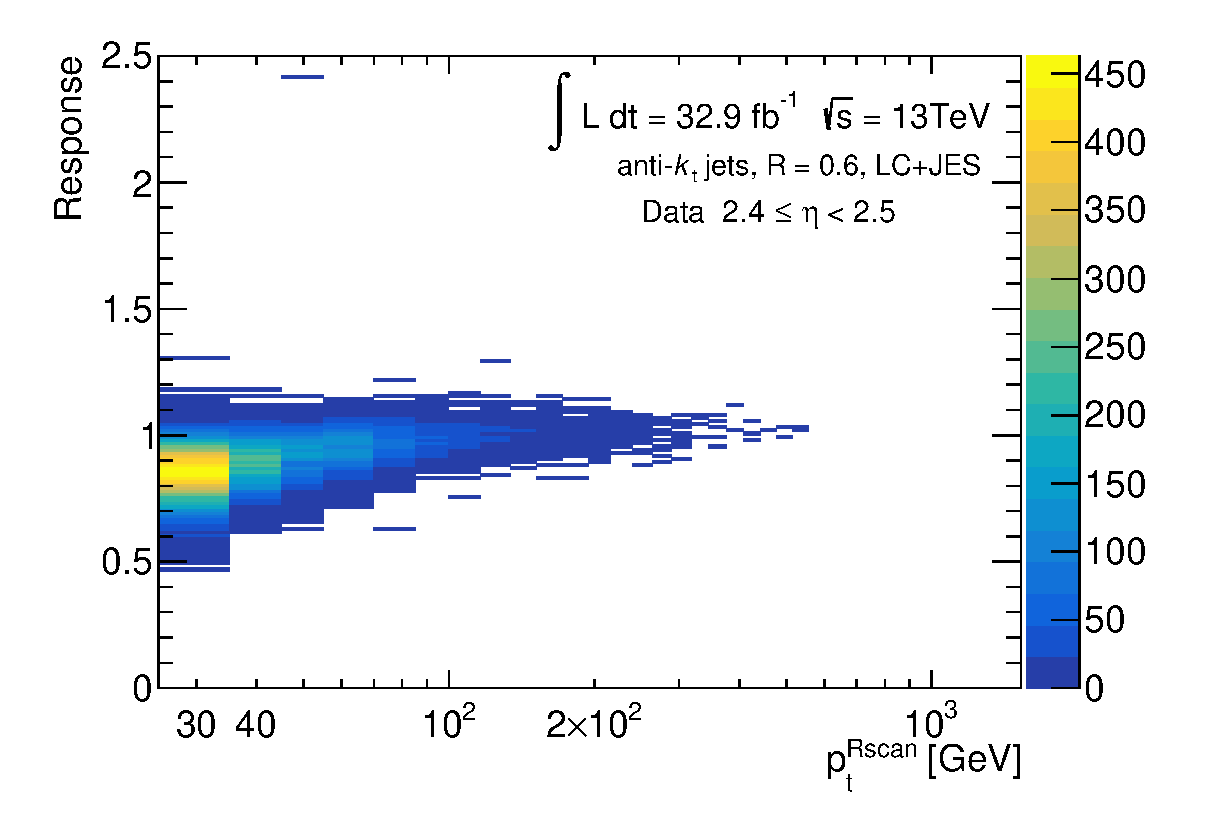
\includegraphics[width=\textwidth]{images/Th2_Data_2lc_eta69}
        \caption{}
        %\label{fig:Th26lc}
    \end{subfigure}
    \hfill
    \begin{subfigure}[b]{0.495\textwidth}
        \centering
        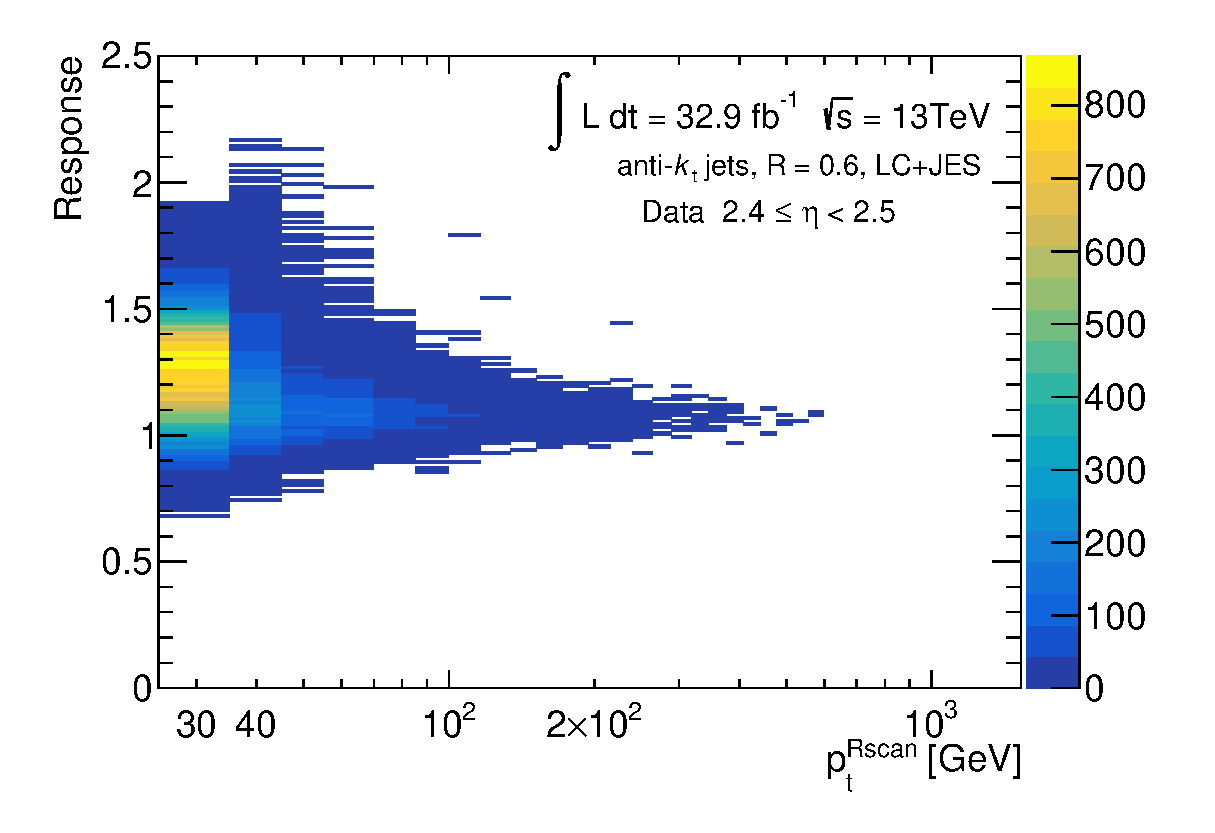
\includegraphics[width=\textwidth]{images/Th2_data_6lc_eta69}
        \caption{}
        %\label{fig:Th26lc}
    \end{subfigure}
    \caption{Distribuciones de la \textit{response} ($\mathcal{R}$) para el bin 0.4$<\eta^{Rscan}_{det}<$0.5 para la colección Rscan con (a) $R_{rscan}=$0.2 y (b) $R_{rscan}=$0.6, y para el bin 2.4$<\eta^{Rscan}_{det}<$2.5 para (c) $R_{rscan}=$0.2 y (d) $R_{rscan}=$0.6 en función de $p_t^{Rscan}$ para el bin de 2.4$<\eta^{Rscan}_{det}<$2.5, en datos recolectados en ATLAS en 2016. La escala de colores da cuenta de las entradas en cada bin.} 
    \label{fig:ResponseTH2}
\end{figure}

\subsection{Análisis}
En los gráficos en la figura \ref{fig:ResponseTH2} se observan algunas tendencias que se repiten tanto en datos como en la simulación y para todos los rangos de $\eta$. La primera a mencionar es que en todos los casos, datos y MC y ambas colecciones de Rscan Jets, la estadística es mayor a bajo momento, siendo máxima en el bin 15 GeV$<p_t^{Rscan}<$20 GeV en el caso de la colección de $R=$0.2 y en el bin  25 GeV$<p_t^{Rscan}<$35 GeV en el caso de la colección de $R=$0.6, y disminuye a medida que aumenta el momento del Rscan Jet. Además, a medida que aumenta el momento del Rscan Jet se observa también que la dispersión de los datos se reduce, y el $\mathcal{R}$ tiende a uno, por valores de $\mathcal{R}$ inferiores para el caso de la colección 0.2 y por encima para el caso de la colección 0.6.
\begin{figure}[ht]
    \centering
    \begin{subfigure}[b]{0.495\textwidth}
        \centering
        \includegraphics[width=\textwidth]{images/Data_2lc_49}
        \caption{Datos}
        %\label{fig:data2lc49}
    \end{subfigure}
    \hfill
    \begin{subfigure}[b]{0.495\textwidth}
        \centering
        \includegraphics[width=\textwidth]{images/MC_2lc_49}
        \caption{MC Powheg+Pythia}
        %\label{fig:Th26lc}
    \end{subfigure}
    \vfill
    \begin{subfigure}[b]{0.495\textwidth}
        \centering
        \includegraphics[width=\textwidth]{images/Data_6lc_49}
        \caption{Datos}
        %\label{fig:Th26lc}
    \end{subfigure}
    \hfill
    \begin{subfigure}[b]{0.495\textwidth}
        \centering
        \includegraphics[width=\textwidth]{images/MC_6lc_49}
        \caption{MC Powheg+Pythia}
        %\label{fig:Th26lc}
    \end{subfigure}
    \caption{ Se muestran los histogramas de \textit{response} y su correspondiente ajuste Gaussiano, indicando con una línea rellena el rango utilizado en el ajuste. Todos los histogramas corresponden al bin 0.4$<\eta^{Rscan}_{det}<$0.5. En el panel superior se muestra el bin 20 GeV$<p_t^{Rscan}<$25 GeV para la colección Rscan con $R_{rscan}=$0.2 en (a) datos de ATLAS 2016 y (b) MC Powheg+Pythia. En el panel inferior se muestra el bin 45 GeV$<p_t^{Rscan}<$55 GeV (c) $R_{rscan}=$0.2 y (d) $R_{rscan}=$0.6 en función de $p_t^{Rscan}$ para la colección con $R_{rscan}=$0.6 en (c) Datos de ATLAS 2016 y (d) MC Powheg+Pythia.} 
    \label{fig:Fits}
\end{figure}

El resto del proceso para derivar la calibración básicamente depende de estos histogramas bidimensionales (y para cada $\eta^{Rscan}_{det}$). Para obtener una calibración (también) en función de $p_t^{Rscan}$, estos histogramas se proyectan en los diferentes bines de $p_t$, obteniéndose histogramas de $\mathcal{R}$ (\textit{response}) para cada bin de $p_t^{Rscan}$ y $\eta_{det}^{Rscan}$. Si bien las distribuciones de \textit{Response} resultan asimétricas, los ajustes gaussianos realizados describen apropiadamente el ``core'' de las distribuciones. En la figura \ref{fig:Fits} se observan algunas distribuciones de $\mathcal{R}$ para un mismo $\eta$ bin tanto, datos como en MC, para ambas colecciones de Rscan Jets. La asimetría mencionada es más pronunciada en el caso de los Rscan Jets con $R=$0.6 en los bines de bajo momento, como se ejemplifica en el panel inferior de la figura \ref{fig:Fits} tanto en datos y en MC. En estas situaciones, se prestó cuidadosa atención a que el ajuste Gaussiano realizado representara adecuadamente el centro de la distribución. En general, la estadística obtenida en las muestras permitió realizar buenos ajustes a partir de $p_t^{Rscan}>$15GeV ($p_t^{Rscan}>$25GeV) y hasta $p_t^{Rscan}\sim$300GeV en la región central $|\eta_{det}^{Rscan}|<$2, disminuyendo el rango hasta $p_t^{Rscan}\sim$200GeV en la región 2$<|\eta_{det}^{Rscan}|<$3, tanto en datos y MC para la colección 0.2 (0.6).  


Con el valor medio que provee el ajuste se mide $<\mathcal{R}>$ en función de $p_t^{Rscan}$ tanto en datos como en MC, para todos los bines de $\eta$ y para ambas colecciones. Finalmente, para cada bin de $\eta$ se toma el cociente entre MC y datos para obtener la corrección ($\mathcal{C}$) a aplicar en los datos. En la figura \ref{fig:Response} se ejemplifica para ambas colecciones de Rscan Jets en los bines 0.4$<\eta^{Rscan}_{det}<$0.5 y 2.4$<\eta^{Rscan}_{det}<$2.5. El error estadístico asociado al valor medio de la response en cada bin corresponde al error con el que el ajuste estima el valor medio de la Gaussiana, y el error en $\mathcal{C}$ resulta de propagar los errores anteriores. 
\begin{figure}[ht]
    \centering
    \begin{subfigure}[b]{0.495\textwidth}
        \centering
        \includegraphics[width=\textwidth]{images/ResponseRatio2LC_49}
        \caption{$R=$0.2 ; 0.4$<\eta^{Rscan}_{det}<$0.5}
        %\label{fig:data2lc49}
    \end{subfigure}
    \hfill
    \begin{subfigure}[b]{0.495\textwidth}
        \centering
        \includegraphics[width=\textwidth]{images/ResponseRatio2LC_69}
        \caption{$R=$0.2 ; 2.4$<\eta^{Rscan}_{det}<$2.5}
        %\label{fig:Th26lc}
    \end{subfigure}
    \vfill
    \begin{subfigure}[b]{0.495\textwidth}
        \centering
        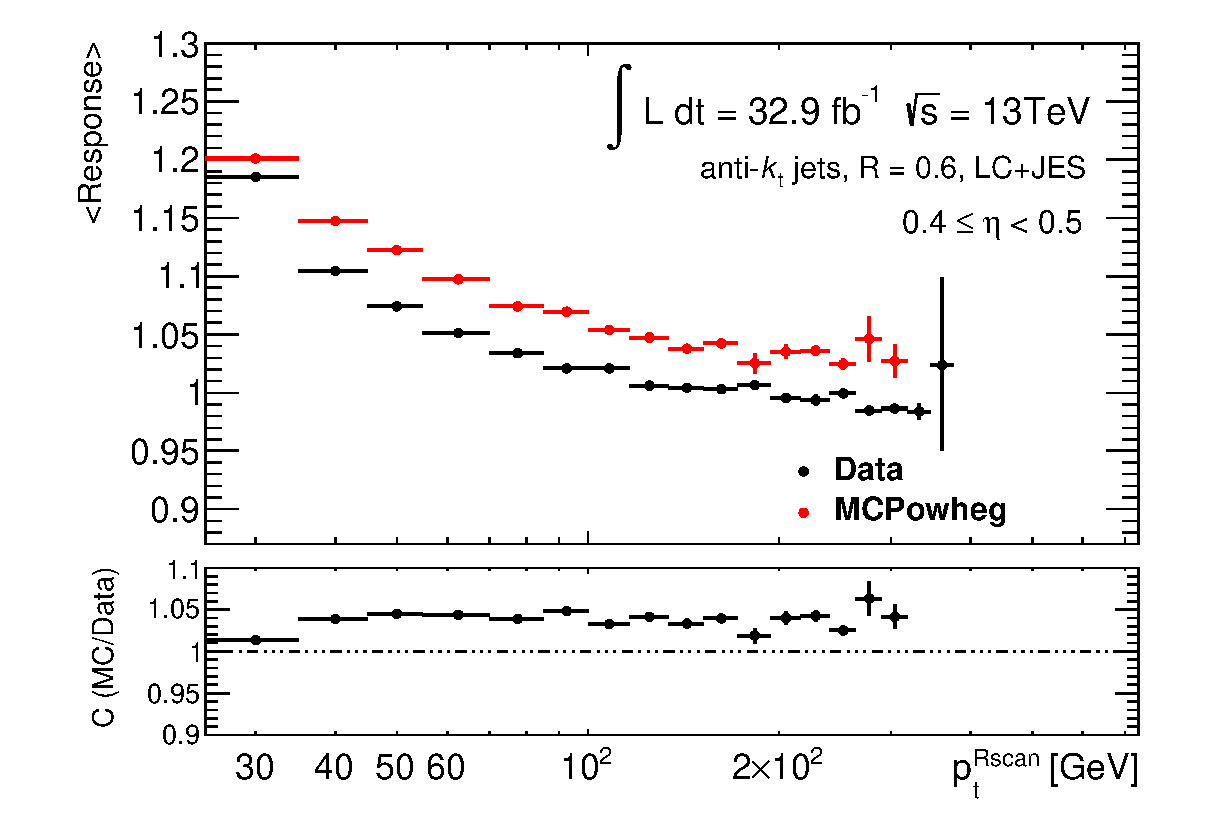
\includegraphics[width=\textwidth]{images/ResponseRatio6LC_49}
        \caption{$R=$0.6 ; 0.4$<\eta^{Rscan}_{det}<$0.5}
        \label{fig:fitFeo}
    \end{subfigure}
    \hfill
    \begin{subfigure}[b]{0.495\textwidth}
        \centering
        \includegraphics[width=\textwidth]{images/ResponseRatio6LC_69}
        \caption{$R=$0.6 ; 2.4$<\eta^{Rscan}_{det}<$2.5}
        %\label{fig:Th26lc}
    \end{subfigure}
    \caption{ Paneles superiores: gráfico del valor medio $<\mathcal{R}>$ en función de $p_t^{Rscan}$ para datos (en negro) recolectados en ATLAS en 2016 y para la muestra nominal, Powheg+Pythia, de MC (en rojo). Paneles inferiores: cociente entre MC y Datos.} 
    \label{fig:Response}
\end{figure}


En la figura \ref{fig:Response} puede observarse una tendencia característica, al igual que en la figura \ref{fig:ResponseTH2}: a medida que aumenta $p_t^{Rscan}$ se observa que $<\mathcal{R}>$ en cada caso comienza a tender hacia un valor estable, por debajo en el caso $R=$0.2, y por encima en el caso $R=$0.6. Observar este crecimiento (decrecimiento) de $<\mathcal{R}>$ en el caso de Rscan Jets con $R=$0.2 (0.6) en datos y MC, pero sobre todo en MC, sugiere que la diferencia en tamaño es la causa. Es decir, en MC los Rscan Jets y los Ref Jets están, prácticamente, calibrados al mismo nivel (no así en datos), por lo que este comportamiento de la response se debe exclusivamente al hecho de haber calibrado los jets con distinto tamaño. Esta tendencia observada en jets aislados podría asociarse con el hecho de que a bajo momento la lluvia de partículas es más ancha y, por lo tanto, al reconstruirla con un jet de radio menor el algoritmo forma el jet de manera diferente y con una menor cantidad de celdas calorimétricas que con un radio mayor, perdiéndose información y reconstruyendo un momento menor en relación al caso de radio mayor.

Además, la tendencia observada en la figura \ref{fig:Response} (y en todos los bines de $\eta$ estudiados) es suave salvo en los últimos bines de momento alcanzados, consistente con el hecho de que a bajo momento se tiene una cantidad de estadística considerablemente mayor, lo que permite hacer un bineado fino en las distribuciones de $\mathcal{R}$ dando más puntos como input al ajuste del core. 

La presencia de algunos puntos con error considerablemente mayor al resto, y desviados de la tendencia general en los gráficos de $\mathcal{R}$, como se ejemplifica en la figura \ref{fig:fitFeo}, se debe, principalmente, a la estadística. Los ajustes gaussianos se realizan de manera automatizada ya que se deben ajustar para cada uno de los 60 bines de $\eta$ más de 30 bines de $p_t$, y esto realizarlo en datos y en MC, y para ambas colecciones de Rscan Jets. Para implementar la automatización, sobre una misma distribución se realizan varios ajustes variando el rango y se toma el mejor ajuste en el sentido de $\chi^2$, pero, a veces, los ajustes que se obtienen no representan adecuadamente a las distribuciones. Por ejemplo, en la figura \ref{fig:DistroFitMalo} se muestra el bin correspondiente 0.4$<\eta^{Rscan}_{det}<$0.5 y 346 GeV$<p^{Rscan}_{t}<$376 GeV para la colección $R=$0.6 en datos, correspondiente a la figura \ref{fig:fitFeo}. Esta figura ejemplifica un caso en el que variar el rango del ajuste, se tiene una mejor calidad en el sentido de $\chi^2$, pero el valor medio obtenido, o mejor dicho el ajuste, no describe apropiadamente la distribución, con lo cual no se debería tener en cuenta ese punto.


\begin{figure}[ht]
    \centering
    \includegraphics[width =0.7\linewidth]{images/FitMalo}
    \caption{Distribución de la response en el bin de 0.4$<\eta^{Rscan}_{det}<$0.5 y 346GeV$<p^{Rscan}_{t}<$376GeV para datos recolectados en ATLAS en 2016. La línea dibujada representa la curva ajustada, la parte rellena indica el rango utilizado para realizar el ajuste Gaussiano. En el rango seleccionado, la curva pasa directamente por los datos, dando un $\chi^2=$0; sin embargo, el ajuste realizado no es representativo de la distribución.}
    \label{fig:DistroFitMalo}
\end{figure}

Las distribuciones de $\mathcal{R}$ obtenidas para datos y la muestra nominal de Powheg+Pythia, en general, tienen buena estadística en el rango de momentos considerado, con lo cual este tipo de fallas rara vez sucede, y cuando sucede lo hace llegando al extremo superior del rango, nuevamente, donde la estadística es menor.\\ 

En el estudio del error sistemático asociado a la elección de un generador de MC se debió trabajar con otra muestra de MC, generada usando \textit{Sherpa} como fue mencionado en la sección \ref{Muestras}. Al repetir este procedimiento utilizando esta muestra se observa que la estadística en las distribuciones de $\mathcal{R}$ es baja en el rango en el que se quiere derivar la calibración. Esto se evidencia en los gráficos de $<\mathcal{R}>$ en función del momento al notar una mayor dispersión de los puntos respecto de la tendencia general observada. Este comportamiento se debe principalmente a que la estadística registrada es mucho menor, en todo el rango de momento estudiado. Esto trae como consecuencia una mayor cantidad de ajustes malos, que ocurren ya en todo el rango y no sólo en el extremo superior como era el caso de datos y Powheg+Pythia, y que deben ser repetidos o estudiados uno por uno. Además, los puntos utilizados para realizar el ajuste tienen asociados un error estadístico mayor. Entonces, de cierta manera, varias curvas pueden ajustar dichos puntos, y por lo tanto, el $<\mathcal{R}>$ se estima con un error mayor. En la figura \ref{fig:ResponseSherpa} se muestran los mismos gráficos que en la figura \ref{fig:Response} pero para el caso en que la muestra de MC corresponde al generador Sherpa.\\    

\begin{figure}[ht]
    \centering
    \begin{subfigure}[b]{0.495\textwidth}
        \centering
        \includegraphics[width=\textwidth]{images/ResponseRatio2LC_49_Sherpa}
        \caption{$R=$0.2 ; 0.4$<\eta^{Rscan}_{det}<$0.5}
        %\label{fig:data2lc49}
    \end{subfigure}
    \hfill
    \begin{subfigure}[b]{0.495\textwidth}
        \centering
        \includegraphics[width=\textwidth]{images/ResponseRatio2LC_69_Sherpa}
        \caption{$R=$0.2 ; 2.4$<\eta^{Rscan}_{det}<$2.5}
        %\label{fig:Th26lc}
    \end{subfigure}
    \vfill
    \begin{subfigure}[b]{0.495\textwidth}
        \centering
        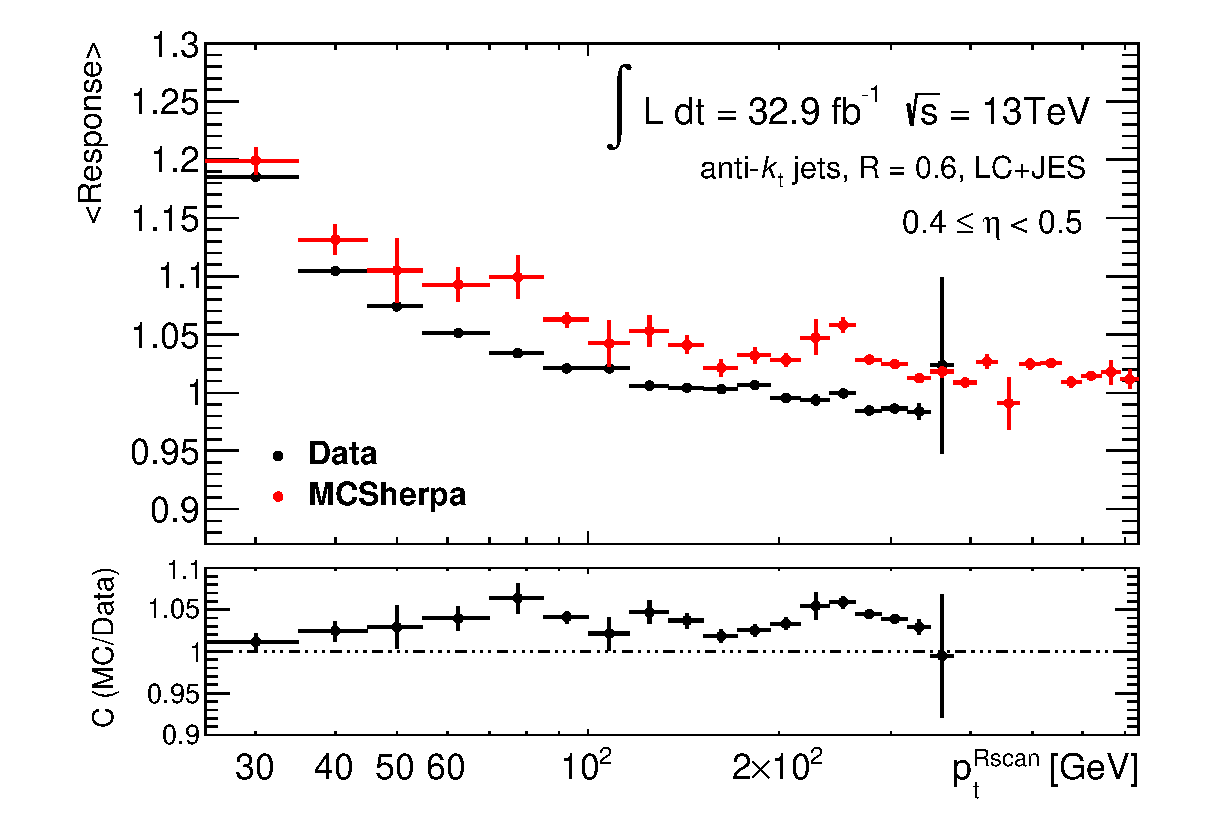
\includegraphics[width=\textwidth]{images/ResponseRatio6LC_49_Sherpa}
        \caption{$R=$0.6 ; 0.4$<\eta^{Rscan}_{det}<$0.5}
        %\label{fig:fitFeo}
    \end{subfigure}
    \hfill
    \begin{subfigure}[b]{0.495\textwidth}
        \centering
        \includegraphics[width=\textwidth]{images/ResponseRatio6LC_69_Sherpa}
        \caption{$R=$0.6 ; 2.4$<\eta^{Rscan}_{det}<$2.5}
        %\label{fig:Th26lc}
    \end{subfigure}
    \caption{ Paneles superiores: gráfico del valor medio $<\mathcal{R}>$ en función de $p_t^{Rscan}$ para datos (en negro) recolectados en ATLAS en 2016 y para la muestra de MC utilizada en el estudio de la incerteza sistemática asociada a la elección de simulación, generada utilizado Sherpa (en rojo). Paneles inferiores: cociente entre MC y Datos.} 
    \label{fig:ResponseSherpa}
\end{figure}

Para reducir el impacto de estas fluctuaciones y anular el de los ajustes malos, se utiliza una técnica de \textit{smoothing} sobre el cociente $\mathcal{C}$, obtenido luego de dividir $<\mathcal{R}>_{MC}$ por $<\mathcal{R}>_{Datos}$. El smoother se aplica en la dirección del momento, para cada bin de $\eta$. La idea del smoother es ajustar los puntos por un promedio pesado, que tiene en cuenta a los puntos vecinos, para obtener una descripción ``suave'' de la tendencia observada. Es decir, sobre un dado bin de $p_t$, el promedio se toma considerando todos los otros bines, donde sus respectivos pesos se asignan con un kernel Gaussiano que tiene en cuenta la distancia al bin considerado. Además, en dicho cálculo también se pesa cada bin por su error asociado.   

\begin{figure}[ht]
    \centering
    \begin{subfigure}[b]{0.495\textwidth}
        \centering
        \includegraphics[width=\textwidth]{images/Smo_2LC_pt_49.png}
        \caption{$R=$0.2 ; 0.4$<\eta^{Rscan}_{det}<$0.5}
        %\label{fig:data2lc49}
    \end{subfigure}
    \hfill
    \begin{subfigure}[b]{0.495\textwidth}
        \centering
        \includegraphics[width=\textwidth]{images/Smo_2LC_pt_69.png}
        \caption{$R=$0.2 ; 2.4$<\eta^{Rscan}_{det}<$2.5}
        %\label{fig:Th26lc}
    \end{subfigure}
    \vfill
    \begin{subfigure}[b]{0.495\textwidth}
        \centering
        \includegraphics[width=\textwidth]{images/Smo_6LC_pt_49.png}
        \caption{$R=$0.6 ; 0.4$<\eta^{Rscan}_{det}<$0.5}
        %\label{fig:fitFeo}
    \end{subfigure}
    \hfill
    \begin{subfigure}[b]{0.495\textwidth}
        \centering
        \includegraphics[width=\textwidth]{images/Smo_6LC_pt_69.png}
        \caption{$R=$0.6 ; 2.4$<\eta^{Rscan}_{det}<$2.5}
        %\label{fig:Th26lc}
    \end{subfigure}
    \caption{ En las figuras se muestra en rojo la corrección y en negro su valor suavizado (en el panel superior), y su cociente (en el panel inferior) en función de $p_t^{Rscan}$ obtenida a partir de datos recolectados en 2016 en ATLAS y usando la muestra nominal de MC, Powheg+Pythia. Las figuras superiores corresponden a la calibración derivada para Rscan Jets de $R=$0.2, y las inferiores para Rscan Jets de $R=$0.6. Las figuras de la izquierda representan un bin de $\eta$ central (0.4$<\eta^{Rscan}_{det}<$0.5) y las de la derecha uno más hacia el extremo del rango consideradp (2.4$<\eta^{Rscan}_{det}<$2.5)} 
    \label{fig:Smoothervspt}
\end{figure}

El uso del smoother debe realizarse con cuidado. La idea detrás de su uso es conseguir una calibración que sea independiente de las fluctuaciones estadísticas observadas. Para ello, se debe identificar una tendencia subyacente en los datos, de manera que la calibración no tenga en cuenta las fluctuaciones específicas de las muestras de estudio, y así cuando se aplique la calibración en otras muestras, no busque reproducirlas. Sin embargo, se debe tener presente que suavizar por demás puede deformar la calibración, perdiéndose la dependencia con el momento. Entonces, de cierta manera el criterio para decidir si el smoother es apropiado, es decir, si suaviza lo suficiente pero no demasiado, es un tanto arbitrario, pero completamente dependiente de la estadística con la que se trabaja. 

\begin{figure}[ht]
    \centering
    \begin{subfigure}[b]{0.495\textwidth}
        \centering
        \includegraphics[width=\textwidth]{images/Smo_2LC_ETA_1.png}
        \caption{$R=$0.2 ; 35GeV$<p_t^{Rscan}<$45GeV}
        %\label{fig:data2lc49}
    \end{subfigure}
    \hfill
    \begin{subfigure}[b]{0.495\textwidth}
        \centering
        \includegraphics[width=\textwidth]{images/Smo_2LC_ETA_2.png}
        \caption{$R=$0.2 ; 85GeV$<p^{Rscan}_t<$100GeV}
        %\label{fig:Th26lc}
    \end{subfigure}
    \vfill
    \begin{subfigure}[b]{0.495\textwidth}
        \centering
        \includegraphics[width=\textwidth]{images/Smo_6LC_ETA_1.png}
        \caption{$R=$0.6 ; 35GeV$<p_t^{Rscan}<$45GeV}
        %\label{fig:fitFeo}
    \end{subfigure}
    \hfill
    \begin{subfigure}[b]{0.495\textwidth}
        \centering
        \includegraphics[width=\textwidth]{images/Smo_6LC_ETA_2.png}
        \caption{$R=$0.6 ; 85GeV$<p^{Rscan}_t<$100GeV}
        %\label{fig:Th26lc}
    \end{subfigure}
    \caption{En las figuras se muestra en rojo la corrección y en negro su valor suavizado (en el panel superior), y su cociente (en el panel inferior) en función de $\eta^{Rscan}_{det}$ obtenida a partir de datos recolectados en 2016 en ATLAS y usando la muestra nominal de MC, Powheg+Pythia. Las figuras superiores corresponden a la calibración derivada para Rscan Jets de $R=$0.2, y las inferiores para Rscan Jets de $R=$0.6. Las figuras de la izquierda representan un bin de $p_t$ bajo (35GeV$<p_t^{Rscan}<$45GeV) y las de la derecha uno mayor (85GeV$<p^{Rscan}_t<$100GeV)} 
    \label{fig:SmoothervsEta}
\end{figure}

En la figura \ref{fig:Smoothervspt} se observa la corrección obtenida en función de $p_t^{Rscan}$ para ambas colecciones en dos bines de $\eta$ y los valores suavizados obtenidos. En el panel inferior de esta figura se observa el cociente entre ambos valores. Para ambos bines de $\eta$ y ambas colecciones se observa que la calibración suavizada sigue fielmente a la corrección derivada, salvo en los últimos bines de momento donde se observa que el cociente difiere de uno, indicando que se han efectivamente suavizado estos factores debido a que en estos puntos el error estadístico es mayor.   

En la figura \ref{fig:SmoothervsEta} se observan los factores de calibración obtenidos, y sus valores suavizados en función de $\eta_{det}$ para dos bines de momento. En esta figura se observa una simetría entre los $\eta$ positivos y los negativos, y una fuerte dependencia con $\eta$, como es de esperarse si se tiene en cuenta la geometría del detector. Se observa también que la corrección aumentará el momento de los Rscan Jets en los bines centrales de $\eta$, y, por el contrario, disminuirá su momento en los bines más externos. 
 
\begin{figure}[ht]
    \centering
    \begin{subfigure}[b]{0.495\textwidth}
        \centering
        \includegraphics[width=\textwidth]{images/Smo_2LC_pt_Sherpa_49.png}
        \caption{$R=$0.2 ; 0.4$<\eta^{Rscan}_{det}<$0.5}
        %\label{fig:data2lc49}
    \end{subfigure}
    \hfill
    \begin{subfigure}[b]{0.495\textwidth}
        \centering
        \includegraphics[width=\textwidth]{images/Smo_2LC_pt_Sherpa_69.png}
        \caption{$R=$0.2 ; 2.4$<\eta^{Rscan}_{det}<$2.5}
        \label{fig:fitMaloSherpa}
    \end{subfigure}
    \vfill
    \begin{subfigure}[b]{0.495\textwidth}
        \centering
        \includegraphics[width=\textwidth]{images/Smo_6LC_pt_49_Sherpa.png}
        \caption{$R=$0.6 ; 0.4$<\eta^{Rscan}_{det}<$0.5}
        %\label{fig:fitFeo}
    \end{subfigure}
    \hfill
    \begin{subfigure}[b]{0.495\textwidth}
        \centering
        \includegraphics[width=\textwidth]{images/Smo_6LC_pt_69_Sherpa.png}
        \caption{$R=$0.6 ; 2.4$<\eta^{Rscan}_{det}<$2.5}
        %\label{fig:Th26lc}
    \end{subfigure}
    \caption{  En las figuras se muestra en rojo la corrección y en negro su valor suavizado (en el panel superior), y su cociente (en el panel inferior) en función de $p_t^{Rscan}$ obtenida a partir de datos recolectados en 2016 en ATLAS y usando la muestra de MC generada en Sherpa para el estudio de la incerteza sistemática. Las figuras superiores corresponden a la calibración derivada para Rscan Jets de $R=$0.2, y las inferiores para Rscan Jets de $R=$0.6. Las figuras de la izquierda representan un bin de $\eta$ central (0.4$<\eta^{Rscan}_{det}<$0.5) y las de la derecha uno más hacia el extremo del rango considerado (2.4$<\eta^{Rscan}_{det}<$2.5).} 
    \label{fig:SmootherSherpa}
\end{figure}

En la figura \ref{fig:SmootherSherpa} se observa la corrección obtenida en función de $p_t$ para ambas colecciones en dos bines de $\eta$ y sus valores suavizados para el caso en que la muestra de MC utilizada fue la generada en Sherpa. En estas figuras se entiende con más claridad la necesidad de utilizar un smoother, ya que los puntos obtenidos presentan una mayor dispersión. En la mismas puede verse también como el método para suavizar beneficia aquellos puntos con menor error estadístico, reduce la influencia de aquellos con error un poco más significativo, y suprime el impacto de puntos como el que se observa en la figura \ref{fig:fitMaloSherpa}, producto de un ajusto malo. 

\begin{comment}
5- R-scan calibration
        - method
        - data and MC samples (paper 13TeV)
        - analysis
            - event selection: 
              - Basic Event Selection on GRID:
                - GRL / Flags / NPV / 
                - Primary Z selection
                  - Muon triggers, muon pt?
                  - weights?
                  - Cutflow: Size of data?
              - Event Cleaning: passLooseBad
              - Z + Jets Selection:
                - Z, muons overlap
                - RefJets & Rscan Jets
              - Isolation 
              - JVT
              - matching    
            - relative response
            - calibration
            - sistematic uncertainties
            - validation
            - comparison with dijet events
\end{comment}

Finalmente, las calibraciones obtenidas para ambas colecciones de jets se presentan, para dos bines de $\eta$ en la figura \ref{fig:FinalCalibration}, junto con su incerteza total, derivada según se explica en la sección \ref{Syst}.

%ctrl +shift + u3e
%ctrl +shift + u3c